\documentclass[twoside]{book}

% Packages required by doxygen
\usepackage{calc}
\usepackage{doxygen}
\usepackage{graphicx}
\usepackage[utf8]{inputenc}
\usepackage{makeidx}
\usepackage{multicol}
\usepackage{multirow}
\usepackage{textcomp}
\usepackage[table]{xcolor}

% Font selection
\usepackage[T1]{fontenc}
\usepackage{mathptmx}
\usepackage[scaled=.90]{helvet}
\usepackage{courier}
\usepackage{amssymb}
\usepackage{sectsty}
\renewcommand{\familydefault}{\sfdefault}
\allsectionsfont{%
  \fontseries{bc}\selectfont%
  \color{darkgray}%
}
\renewcommand{\DoxyLabelFont}{%
  \fontseries{bc}\selectfont%
  \color{darkgray}%
}

% Page & text layout
\usepackage{geometry}
\geometry{%
  a4paper,%
  top=2.5cm,%
  bottom=2.5cm,%
  left=2.5cm,%
  right=2.5cm%
}
\tolerance=750
\hfuzz=15pt
\hbadness=750
\setlength{\emergencystretch}{15pt}
\setlength{\parindent}{0cm}
\setlength{\parskip}{0.2cm}
\makeatletter
\renewcommand{\paragraph}{%
  \@startsection{paragraph}{4}{0ex}{-1.0ex}{1.0ex}{%
    \normalfont\normalsize\bfseries\SS@parafont%
  }%
}
\renewcommand{\subparagraph}{%
  \@startsection{subparagraph}{5}{0ex}{-1.0ex}{1.0ex}{%
    \normalfont\normalsize\bfseries\SS@subparafont%
  }%
}
\makeatother

% Headers & footers
\usepackage{fancyhdr}
\pagestyle{fancyplain}
\fancyhead[LE]{\fancyplain{}{\bfseries\thepage}}
\fancyhead[CE]{\fancyplain{}{}}
\fancyhead[RE]{\fancyplain{}{\bfseries\leftmark}}
\fancyhead[LO]{\fancyplain{}{\bfseries\rightmark}}
\fancyhead[CO]{\fancyplain{}{}}
\fancyhead[RO]{\fancyplain{}{\bfseries\thepage}}
\fancyfoot[LE]{\fancyplain{}{}}
\fancyfoot[CE]{\fancyplain{}{}}
\fancyfoot[RE]{\fancyplain{}{\bfseries\scriptsize Generated on Mon Oct 5 2015 16\-:28\-:10 for L\-I\-F\-T -\/ Lift Is not a Framework or Toolkit by Doxygen }}
\fancyfoot[LO]{\fancyplain{}{\bfseries\scriptsize Generated on Mon Oct 5 2015 16\-:28\-:10 for L\-I\-F\-T -\/ Lift Is not a Framework or Toolkit by Doxygen }}
\fancyfoot[CO]{\fancyplain{}{}}
\fancyfoot[RO]{\fancyplain{}{}}
\renewcommand{\footrulewidth}{0.4pt}
\renewcommand{\chaptermark}[1]{%
  \markboth{#1}{}%
}
\renewcommand{\sectionmark}[1]{%
  \markright{\thesection\ #1}%
}

% Indices & bibliography
\usepackage{natbib}
\usepackage[titles]{tocloft}
\setcounter{tocdepth}{3}
\setcounter{secnumdepth}{5}
\makeindex

% Hyperlinks (required, but should be loaded last)
\usepackage{ifpdf}
\ifpdf
  \usepackage[pdftex,pagebackref=true]{hyperref}
\else
  \usepackage[ps2pdf,pagebackref=true]{hyperref}
\fi
\hypersetup{%
  colorlinks=true,%
  linkcolor=blue,%
  citecolor=blue,%
  unicode%
}

% Custom commands
\newcommand{\clearemptydoublepage}{%
  \newpage{\pagestyle{empty}\cleardoublepage}%
}


%===== C O N T E N T S =====

\begin{document}

% Titlepage & ToC
\hypersetup{pageanchor=false}
\pagenumbering{roman}
\begin{titlepage}
\vspace*{7cm}
\begin{center}%
{\Large L\-I\-F\-T -\/ Lift Is not a Framework or Toolkit }\\
\vspace*{1cm}
{\large Generated by Doxygen 1.8.6}\\
\vspace*{0.5cm}
{\small Mon Oct 5 2015 16:28:10}\\
\end{center}
\end{titlepage}
\clearemptydoublepage
\tableofcontents
\clearemptydoublepage
\pagenumbering{arabic}
\hypersetup{pageanchor=true}

%--- Begin generated contents ---
\chapter{L\-I\-F\-T}
\label{index}\hypertarget{index}{}L\-I\-F\-T is a collectiong of useful C modules. It isn't a framework or a Toolkit. Most modules are either self-\/sufficient (depend only on parts of C standard library, or, in some cases, parts of standard library for a given system (P\-O\-S\-I\-X, Windows...)), or depend on a few other L\-I\-F\-T modules.

For a reasonably type-\/safe realloc for arrays (and, in most cases you use realloc for arrays), check out \hyperlink{lift__arealloc_8h}{lift\-\_\-arealloc.\-h}.

For a reasonably type-\/safe free that also N\-U\-L\-L-\/ifies the pointer, check out \hyperlink{lift__free__and__null_8h}{lift\-\_\-free\-\_\-and\-\_\-null.\-h}.

For a reasonably type-\/safe and efficient generic vector, with an interface inspired by C++ S\-T\-L, check out \hyperlink{lift__vec_8h}{lift\-\_\-vec.\-h}.

For a minimalistic, type-\/safe and efficient generic list, with interface having no resemblense of C++ S\-T\-L, check out \hyperlink{lift__list_8h}{lift\-\_\-list.\-h}. 
\chapter{lift-\/c}
\label{md_README}
\hypertarget{md_README}{}
This is a bunch of useful C modules. The name of this kind-\/of-\/library, \char`\"{}\-L\-I\-F\-T\char`\"{}, can be interpreted as a recursive acronym\-: Lift Is not a Framework or a Toolkit (a bunch of useful C modules).

Also, it is a slight pun on a well-\/known C++ library. This is C, we don't need a {\itshape boost} we just need a {\itshape lift}. \-:)

\subsection*{What is there}

Well, there is the \char`\"{}master\char`\"{} include file {\ttfamily \hyperlink{lift_8h}{lift.\-h}}, but, in most cases, you should just include the header of the module that you need. 
\chapter{File Index}
\section{File List}
Here is a list of all documented files with brief descriptions\-:\begin{DoxyCompactList}
\item\contentsline{section}{\hyperlink{lift_8h}{lift.\-h} }{\pageref{lift_8h}}{}
\item\contentsline{section}{\hyperlink{lift__arealloc_8h}{lift\-\_\-arealloc.\-h} \\*Safe alternative for realloc() for arrays }{\pageref{lift__arealloc_8h}}{}
\item\contentsline{section}{\hyperlink{lift__free__and__null_8h}{lift\-\_\-free\-\_\-and\-\_\-null.\-h} \\*A safer alternative to free() }{\pageref{lift__free__and__null_8h}}{}
\item\contentsline{section}{\hyperlink{lift__vec_8h}{lift\-\_\-vec.\-h} \\*A vector generic type for C }{\pageref{lift__vec_8h}}{}
\end{DoxyCompactList}

\chapter{File Documentation}
\hypertarget{lift_8h}{\section{lift.\-h File Reference}
\label{lift_8h}\index{lift.\-h@{lift.\-h}}
}
{\ttfamily \#include \char`\"{}lift\-\_\-arealloc.\-h\char`\"{}}\\*
Include dependency graph for lift.\-h\-:\nopagebreak
\begin{figure}[H]
\begin{center}
\leavevmode
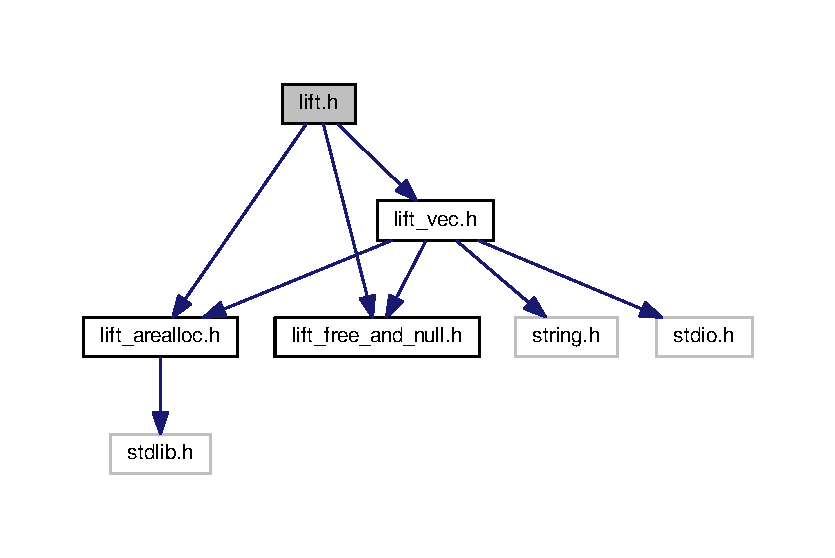
\includegraphics[width=154pt]{lift_8h__incl}
\end{center}
\end{figure}

\hypertarget{lift__arealloc_8h}{\section{lift\-\_\-arealloc.\-h File Reference}
\label{lift__arealloc_8h}\index{lift\-\_\-arealloc.\-h@{lift\-\_\-arealloc.\-h}}
}


Safe alternative for realloc() for arrays.  


{\ttfamily \#include $<$stdlib.\-h$>$}\\*
Include dependency graph for lift\-\_\-arealloc.\-h\-:\nopagebreak
\begin{figure}[H]
\begin{center}
\leavevmode
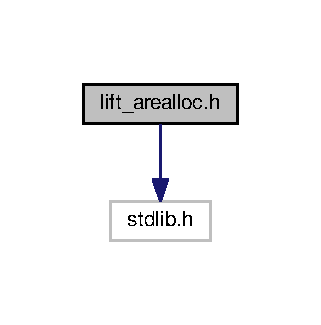
\includegraphics[width=154pt]{lift__arealloc_8h__incl}
\end{center}
\end{figure}
This graph shows which files directly or indirectly include this file\-:\nopagebreak
\begin{figure}[H]
\begin{center}
\leavevmode
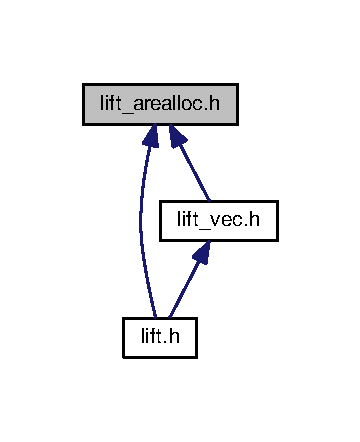
\includegraphics[width=189pt]{lift__arealloc_8h__dep__incl}
\end{center}
\end{figure}
\subsection*{Macros}
\begin{DoxyCompactItemize}
\item 
\#define \hyperlink{lift__arealloc_8h_aa29066af0304aa4445b7e13ccff595de}{lift\-\_\-arealloc}(ptr, members)~\hyperlink{lift__arealloc_8h_a2193a6bf115f8542b19f0225cfb6a306}{lift\-\_\-arealloc\-\_\-implementation}(\&(ptr),(members), sizeof $\ast$(ptr))
\begin{DoxyCompactList}\small\item\em This macro makes lif\-\_\-arealloc\-\_\-implementation() a lot easier to use and less error prone. \end{DoxyCompactList}\end{DoxyCompactItemize}
\subsection*{Functions}
\begin{DoxyCompactItemize}
\item 
void $\ast$ \hyperlink{lift__arealloc_8h_a2193a6bf115f8542b19f0225cfb6a306}{lift\-\_\-arealloc\-\_\-implementation} (void $\ast$ptrptr, size\-\_\-t members, size\-\_\-t size)
\begin{DoxyCompactList}\small\item\em A safe alternative to realloc() for arrays. \end{DoxyCompactList}\end{DoxyCompactItemize}


\subsection{Detailed Description}
Safe alternative for realloc() for arrays. Part of L\-I\-F\-T, but can be used on its own -\/ doesn't depend on anything from L\-I\-F\-T. \begin{DoxyAuthor}{Author}
Srdjan Veljkovic 
\end{DoxyAuthor}
\begin{DoxyCopyright}{Copyright}
M\-I\-T License 
\end{DoxyCopyright}


\subsection{Macro Definition Documentation}
\hypertarget{lift__arealloc_8h_aa29066af0304aa4445b7e13ccff595de}{\index{lift\-\_\-arealloc.\-h@{lift\-\_\-arealloc.\-h}!lift\-\_\-arealloc@{lift\-\_\-arealloc}}
\index{lift\-\_\-arealloc@{lift\-\_\-arealloc}!lift_arealloc.h@{lift\-\_\-arealloc.\-h}}
\subsubsection[{lift\-\_\-arealloc}]{\setlength{\rightskip}{0pt plus 5cm}\#define lift\-\_\-arealloc(
\begin{DoxyParamCaption}
\item[{}]{ptr, }
\item[{}]{members}
\end{DoxyParamCaption}
)~{\bf lift\-\_\-arealloc\-\_\-implementation}(\&(ptr),(members), sizeof $\ast$(ptr))}}\label{lift__arealloc_8h_aa29066af0304aa4445b7e13ccff595de}


This macro makes lif\-\_\-arealloc\-\_\-implementation() a lot easier to use and less error prone. 

It is a {\itshape good} macro, as it is very simple and doesn't evaluate its arguments more than once.

We fix two usability issues\-:
\begin{DoxyEnumerate}
\item You may pass a pointer (to a value) instead of a pointer to pointer
\item You may pass a wrong (element) size
\end{DoxyEnumerate}

Here we accept a pointer, and you can't pass a value. You can, of course pass a pointer to pointer, but, that may be valid input, so we can't reject that.

The size of an element is deduced to be {\ttfamily sizeof $\ast$ptr}.


\begin{DoxyParams}{Parameters}
{\em ptr} & The pointer to reallocate -\/ it will be changed \char`\"{}in place\char`\"{}, if need be. \\
\hline
{\em members} & The number of members of the new array \\
\hline
\end{DoxyParams}
\begin{DoxyReturn}{Returns}
Pointer to the new array or N\-U\-L\-L on failure to (re)allocate 
\end{DoxyReturn}
\begin{Desc}
\item[Examples\-: ]\par
\hyperlink{lift_arealloc_example_8c-example}{lift\-\_\-arealloc\-\_\-example.\-c}.\end{Desc}


\subsection{Function Documentation}
\hypertarget{lift__arealloc_8h_a2193a6bf115f8542b19f0225cfb6a306}{\index{lift\-\_\-arealloc.\-h@{lift\-\_\-arealloc.\-h}!lift\-\_\-arealloc\-\_\-implementation@{lift\-\_\-arealloc\-\_\-implementation}}
\index{lift\-\_\-arealloc\-\_\-implementation@{lift\-\_\-arealloc\-\_\-implementation}!lift_arealloc.h@{lift\-\_\-arealloc.\-h}}
\subsubsection[{lift\-\_\-arealloc\-\_\-implementation}]{\setlength{\rightskip}{0pt plus 5cm}void$\ast$ lift\-\_\-arealloc\-\_\-implementation (
\begin{DoxyParamCaption}
\item[{void $\ast$}]{ptrptr, }
\item[{size\-\_\-t}]{members, }
\item[{size\-\_\-t}]{size}
\end{DoxyParamCaption}
)}}\label{lift__arealloc_8h_a2193a6bf115f8542b19f0225cfb6a306}


A safe alternative to realloc() for arrays. 

It avoids the problems of overflow ({\ttfamily members} $\ast$  may overflow) and \char`\"{}leaking\char`\"{} the previously allocated memory in case of failure. In case you're not aware of it, here is the offending code\-: \begin{DoxyVerb}char *s = malloc(100);
s = realloc(s, 200);
\end{DoxyVerb}


If realloc() fails, {\ttfamily s} will now be N\-U\-L\-L, and previously malloc()-\/ ated memory is leaked, there is no way to free it now.

The only problem that \hyperlink{lift__arealloc_8h_aa29066af0304aa4445b7e13ccff595de}{lift\-\_\-arealloc()} doesn't solve is that passing an invalid pointer (not N\-U\-L\-L or \char`\"{}really\char`\"{} allocated) results in undefined behavior.

\begin{DoxyWarning}{Warning}
Don't forget to pass the address of your pointer, rather than the pointer itself, even though the formal parameter type for  is {\ttfamily void$\ast$}.
\end{DoxyWarning}
So, to fix the realloc() problem cited above, we would\-: \begin{DoxyVerb}char *s = malloc(100);
if (NULL == lift_arealloc(&s, 200, sizeof(char)) {
    // handle reallocation failure, but `s` stayed the same
}
\end{DoxyVerb}


\begin{DoxyNote}{Note}
The downside is that may simply forget to pass the address of your pointer, and pass the pointer itself, and there is no way that we can detect that. Declaring {\ttfamily ptrptr} to be a {\ttfamily void$\ast$$\ast$} would have actually been worse, as that would require cast if you want to avoid warnings (or even errors) for passing a pointer to, say, {\ttfamily int$\ast$}, instead of to {\ttfamily void$\ast$}. So, passing something like {\ttfamily 3}, because you cast it to {\ttfamily void$\ast$$\ast$} would not be detected.
\end{DoxyNote}
To help with these usability issues, you should probably use \hyperlink{lift__arealloc_8h_aa29066af0304aa4445b7e13ccff595de}{lift\-\_\-arealloc} macro instead of this function.

\begin{DoxyRemark}{Remarks}
On detecting overflow or any other invalid usage, it will {\itshape not} call realloc and will return N\-U\-L\-L and set {\ttfamily errno} to E\-R\-A\-N\-G\-E. If realloc() returns N\-U\-L\-L, {\ttfamily ptrptr} will not be changed. Otherwise, the result of realloc() will be written to {\ttfamily $\ast$ptrptr}.
\end{DoxyRemark}

\begin{DoxyParams}[1]{Parameters}
\mbox{\tt in,out}  & {\em ptrptr} & Pointer to pointer to be reallocated. N\-U\-L\-L is invalid. If not N\-U\-L\-L, and other checks pass, {\ttfamily $\ast$ptrptr} will passed to realloc().\\
\hline
\mbox{\tt in}  & {\em members} & The number of members of the new array. If the result of multiply with {\ttfamily size} doesn't overflow, that result will be passed to realloc(). Also, if it or  is 0, the function may fail.\\
\hline
\mbox{\tt in}  & {\em size} & Size of a member of the new array. If the result of multiply with {\ttfamily members} doesn't overflow, that result will be passed to realloc(). Also, if it or  is 0, the function may fail.\\
\hline
\end{DoxyParams}
\begin{DoxyReturn}{Returns}
On internal or realloc() failure, will return N\-U\-L\-L. Otherwise, will return the result of realloc(). 
\end{DoxyReturn}
\begin{Desc}
\item[Examples\-: ]\par
\hyperlink{lift_arealloc_example_8c-example}{lift\-\_\-arealloc\-\_\-example.\-c}.\end{Desc}

\hypertarget{lift__free__and__null_8h}{\section{lift\-\_\-free\-\_\-and\-\_\-null.\-h File Reference}
\label{lift__free__and__null_8h}\index{lift\-\_\-free\-\_\-and\-\_\-null.\-h@{lift\-\_\-free\-\_\-and\-\_\-null.\-h}}
}


A safer alternative to free().  


This graph shows which files directly or indirectly include this file\-:
\nopagebreak
\begin{figure}[H]
\begin{center}
\leavevmode
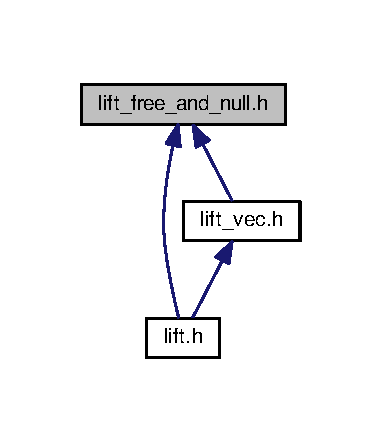
\includegraphics[width=184pt]{lift__free__and__null_8h__dep__incl}
\end{center}
\end{figure}
\subsection*{Macros}
\begin{DoxyCompactItemize}
\item 
\#define \hyperlink{lift__free__and__null_8h_ae429d1e4d6d8ae834f8174d6cf0b9e10}{lift\-\_\-nfree}(ptr)~\hyperlink{lift__free__and__null_8h_a873930b05bedfabc4dadf6df93a88428}{lift\-\_\-free\-\_\-and\-\_\-null}(\&(ptr)), sizeof $\ast$(ptr)
\begin{DoxyCompactList}\small\item\em This macro solves the usability problem with \hyperlink{lift__free__and__null_8h_a873930b05bedfabc4dadf6df93a88428}{lift\-\_\-free\-\_\-and\-\_\-null()}. \end{DoxyCompactList}\end{DoxyCompactItemize}
\subsection*{Functions}
\begin{DoxyCompactItemize}
\item 
void \hyperlink{lift__free__and__null_8h_a873930b05bedfabc4dadf6df93a88428}{lift\-\_\-free\-\_\-and\-\_\-null} (void $\ast$ptrptr)
\begin{DoxyCompactList}\small\item\em An alternative / wrapper to free(). \end{DoxyCompactList}\end{DoxyCompactItemize}


\subsection{Detailed Description}
A safer alternative to free(). \begin{DoxyAuthor}{Author}
Srdjan Veljkovic 
\end{DoxyAuthor}
\begin{DoxyCopyright}{Copyright}
M\-I\-T license 
\end{DoxyCopyright}


\subsection{Macro Definition Documentation}
\hypertarget{lift__free__and__null_8h_ae429d1e4d6d8ae834f8174d6cf0b9e10}{\index{lift\-\_\-free\-\_\-and\-\_\-null.\-h@{lift\-\_\-free\-\_\-and\-\_\-null.\-h}!lift\-\_\-nfree@{lift\-\_\-nfree}}
\index{lift\-\_\-nfree@{lift\-\_\-nfree}!lift_free_and_null.h@{lift\-\_\-free\-\_\-and\-\_\-null.\-h}}
\subsubsection[{lift\-\_\-nfree}]{\setlength{\rightskip}{0pt plus 5cm}\#define lift\-\_\-nfree(
\begin{DoxyParamCaption}
\item[{}]{ptr}
\end{DoxyParamCaption}
)~{\bf lift\-\_\-free\-\_\-and\-\_\-null}(\&(ptr)), sizeof $\ast$(ptr)}}\label{lift__free__and__null_8h_ae429d1e4d6d8ae834f8174d6cf0b9e10}


This macro solves the usability problem with \hyperlink{lift__free__and__null_8h_a873930b05bedfabc4dadf6df93a88428}{lift\-\_\-free\-\_\-and\-\_\-null()}. 

It is a {\itshape good} macro, as it is simple and does not evaluate its argument more than once.

Here we expect a pointer and you can't pass a variable. Of course, you may pass a pointer to pointer, but that may be valid input.

There is an additional check -\/ you can't pass a void pointer. That means that some strange, but valid code, will not compile. If you have such code, use \hyperlink{lift__free__and__null_8h_a873930b05bedfabc4dadf6df93a88428}{lift\-\_\-free\-\_\-and\-\_\-null()}, but be careful.


\begin{DoxyParams}{Parameters}
{\em ptr} & The pointer to free (previously allocated by malloc() or realloc()). It will be set to N\-U\-L\-L \char`\"{}in place\char`\"{} \\
\hline
\end{DoxyParams}
\begin{DoxyReturn}{Returns}
The size of what the {\ttfamily ptr} points to 
\end{DoxyReturn}
\begin{Desc}
\item[Examples\-: ]\par
\hyperlink{lift_free_and_null_example_8c-example}{lift\-\_\-free\-\_\-and\-\_\-null\-\_\-example.\-c}.\end{Desc}


\subsection{Function Documentation}
\hypertarget{lift__free__and__null_8h_a873930b05bedfabc4dadf6df93a88428}{\index{lift\-\_\-free\-\_\-and\-\_\-null.\-h@{lift\-\_\-free\-\_\-and\-\_\-null.\-h}!lift\-\_\-free\-\_\-and\-\_\-null@{lift\-\_\-free\-\_\-and\-\_\-null}}
\index{lift\-\_\-free\-\_\-and\-\_\-null@{lift\-\_\-free\-\_\-and\-\_\-null}!lift_free_and_null.h@{lift\-\_\-free\-\_\-and\-\_\-null.\-h}}
\subsubsection[{lift\-\_\-free\-\_\-and\-\_\-null}]{\setlength{\rightskip}{0pt plus 5cm}void lift\-\_\-free\-\_\-and\-\_\-null (
\begin{DoxyParamCaption}
\item[{void $\ast$}]{ptrptr}
\end{DoxyParamCaption}
)}}\label{lift__free__and__null_8h_a873930b05bedfabc4dadf6df93a88428}


An alternative / wrapper to free(). 

It will N\-U\-L\-L the pointer, not just free() it. Thus, you will not have a dangling pointer.

Passing N\-U\-L\-L or a pointer to N\-U\-L\-L (pointer) will simply be ignored. Otherwise, free() will be called on {\ttfamily $\ast$ptrptr} and then it will be N\-U\-L\-L-\/ed.

\begin{DoxyWarning}{Warning}
You must pass the address of your pointer, not the pointer itself. Since {\ttfamily ptrptr} is of {\ttfamily void$\ast$}, it will not detect if you pass the pointer, and we shall have undefined behavior.
\end{DoxyWarning}
\begin{DoxyRemark}{Remarks}
The advantage of this function versus a pure macro implementation is that we avoid the problem of multiple evaluation in the macro. That should make it easier to find bugs with not passing address of a pointer (but the pointer itself).
\end{DoxyRemark}
We provida macro wrapper in \hyperlink{lift__free__and__null_8h_ae429d1e4d6d8ae834f8174d6cf0b9e10}{lift\-\_\-nfree}, that solves this usability problem.

\begin{DoxyRemark}{Remarks}
Declaring {\ttfamily ptrptr} to be of {\ttfamily void $\ast$$\ast$} type would be much worse, as to silence warnings (or maybe errors) one would need to cast to {\ttfamily void$\ast$$\ast$} always, which would enable passing {\itshape anything}.
\end{DoxyRemark}

\begin{DoxyParams}[1]{Parameters}
\mbox{\tt in,out}  & {\em ptrptr} & Pointer to the pointer to free and N\-U\-L\-L \\
\hline
\end{DoxyParams}
\begin{Desc}
\item[Examples\-: ]\par
\hyperlink{lift_free_and_null_example_8c-example}{lift\-\_\-free\-\_\-and\-\_\-null\-\_\-example.\-c}.\end{Desc}

\chapter{Example Documentation}
\hypertarget{lift_arealloc_example_8c-example}{\section{lift\-\_\-arealloc\-\_\-example.\-c}
}

\begin{DoxyCodeInclude}
\textcolor{comment}{/* -*- c-file-style:"stroustrup"; indent-tabs-mode: nil -*- */}
\textcolor{preprocessor}{#include "\hyperlink{lift__arealloc_8h}{lift\_arealloc.h}"}

\textcolor{preprocessor}{#include <stdio.h>}
\textcolor{preprocessor}{#include <assert.h>}


\textcolor{keywordtype}{int} main()
\{
    \textcolor{keywordtype}{int} *v = NULL;
    \textcolor{keywordflow}{if} (NULL == \hyperlink{lift__arealloc_8h_a2193a6bf115f8542b19f0225cfb6a306}{lift\_arealloc\_implementation}(&v, 4, \textcolor{keyword}{sizeof} *v)) \{
        printf(\textcolor{stringliteral}{"Failed to allocate memory\(\backslash\)n"});
        \textcolor{keywordflow}{return} -1;
    \}
    v[0] = v[1] = v[2] = v[3] = 4443;

    \textcolor{keywordflow}{if} (NULL == \hyperlink{lift__arealloc_8h_a2193a6bf115f8542b19f0225cfb6a306}{lift\_arealloc\_implementation}(&v, 8, \textcolor{keyword}{sizeof} *v)) \{
        printf(\textcolor{stringliteral}{"Failed to re-allocate memory\(\backslash\)n"});
    \textcolor{keywordflow}{return} -1;
    \}
    \textcolor{keywordflow}{if} (NULL == \hyperlink{lift__arealloc_8h_a2193a6bf115f8542b19f0225cfb6a306}{lift\_arealloc\_implementation}(&v, (\textcolor{keywordtype}{size\_t})~0, \textcolor{keyword}{sizeof} *v)) \{
        printf(\textcolor{stringliteral}{"Failed to re-allocate memory, as expected\(\backslash\)n"});
    \}
    v[4] = v[5] = v[6] = v[7] = 443;

    \textcolor{keywordflow}{if} (NULL == \hyperlink{lift__arealloc_8h_aa29066af0304aa4445b7e13ccff595de}{lift\_arealloc}(v, 6)) \{
        printf(\textcolor{stringliteral}{"Failed to re-allocate memory\(\backslash\)n"});
    \textcolor{keywordflow}{return} -1;
    \}
    \textcolor{keywordflow}{if} (NULL == \hyperlink{lift__arealloc_8h_aa29066af0304aa4445b7e13ccff595de}{lift\_arealloc}(v, (\textcolor{keywordtype}{size\_t})~0)) \{
        printf(\textcolor{stringliteral}{"Failed to re-allocate memory, as expected\(\backslash\)n"});
    \}

    assert(v[5] == 443);

    free(v);

    puts(\textcolor{stringliteral}{"lift\_arealloc() example finished normally"});

    \textcolor{keywordflow}{return} 0;
\}
\end{DoxyCodeInclude}
 
\hypertarget{lift_free_and_null_example_8c-example}{\section{lift\-\_\-free\-\_\-and\-\_\-null\-\_\-example.\-c}
}

\begin{DoxyCodeInclude}
\textcolor{preprocessor}{#include "\hyperlink{lift__free__and__null_8h}{lift\_free\_and\_null.h}"}

\textcolor{preprocessor}{#include <stdio.h>}
\textcolor{preprocessor}{#include <stdlib.h>}


\textcolor{keywordtype}{int} main()
\{
    \textcolor{keywordtype}{char} *s = malloc(100);
    printf(\textcolor{stringliteral}{"s = %p; after malloc()\(\backslash\)n"}, s);
    free(s);
    printf(\textcolor{stringliteral}{"s = %p; after free()\(\backslash\)n"}, s);

    s = malloc(1000);
    printf(\textcolor{stringliteral}{"s = %p; after another malloc()\(\backslash\)n"}, s);
    \hyperlink{lift__free__and__null_8h_a873930b05bedfabc4dadf6df93a88428}{lift\_free\_and\_null}(&s);
    printf(\textcolor{stringliteral}{"s = %p; after lift\_free\_and\_null()\(\backslash\)n"}, s);

    s = malloc(10000);
    printf(\textcolor{stringliteral}{"s = %p; after yet another malloc()\(\backslash\)n"}, s);
    \hyperlink{lift__free__and__null_8h_ae429d1e4d6d8ae834f8174d6cf0b9e10}{lift\_nfree}(s+2);
    printf(\textcolor{stringliteral}{"s = %p; after lift\_nfree()\(\backslash\)n"}, s);

    \textcolor{keywordflow}{return} 0;
\}
\end{DoxyCodeInclude}
 
%--- End generated contents ---

% Index
\newpage
\phantomsection
\addcontentsline{toc}{chapter}{Index}
\printindex

\end{document}
